\begin{center}


\tikzset{every picture/.style={line width=0.75pt}} %set default line width to 0.75pt        

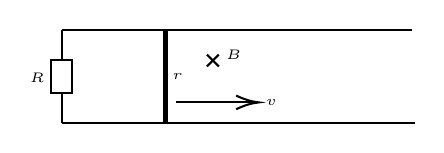
\begin{tikzpicture}[x=0.75pt,y=0.75pt,yscale=-1,xscale=1]
%uncomment if require: \path (0,300); %set diagram left start at 0, and has height of 300

%Straight Lines [id:da0541029549392007] 
\draw    (100,105) -- (269,105) ;
%Straight Lines [id:da4496264717956384] 
\draw    (100,150) -- (270,150) ;
%Shape: Resistor [id:dp8047057543211917] 
\draw   (105,119.71) -- (105,135.55) -- (95,135.55) -- (95,119.71) -- (105,119.71) -- cycle (100,115.25) -- (100,119.71) (100,135.55) -- (100,140) ;
%Straight Lines [id:da051255858179573455] 
\draw    (100,115.25) -- (100,105) ;
%Straight Lines [id:da7781373986650673] 
\draw    (100,150) -- (100,139.75) ;
%Straight Lines [id:da17409470417502937] 
\draw [line width=1.5]    (150,105) -- (150,150) ;
%Straight Lines [id:da5329011887831403] 
\draw    (155,140) -- (193,140) ;
\draw [shift={(195,140)}, rotate = 180] [color={rgb, 255:red, 0; green, 0; blue, 0 }  ][line width=0.75]    (10.93,-3.29) .. controls (6.95,-1.4) and (3.31,-0.3) .. (0,0) .. controls (3.31,0.3) and (6.95,1.4) .. (10.93,3.29)   ;
%Straight Lines [id:da6865175298817716] 
\draw    (170,117) -- (175.7,122.7) ;
%Straight Lines [id:da3716548751829467] 
\draw    (175.7,117) -- (170,122.7) ;


% Text Node
\draw (93,132.15) node [anchor=south east] [inner sep=0.75pt]  [font=\tiny]  {$R$};
% Text Node
\draw (152,127.5) node [anchor=west] [inner sep=0.75pt]  [font=\tiny]  {$r$};
% Text Node
\draw (197,140) node [anchor=west] [inner sep=0.75pt]  [font=\tiny]  {$v$};
% Text Node
\draw (177.7,117) node [anchor=west] [inner sep=0.75pt]  [font=\tiny]  {$B$};


\end{tikzpicture}

\end{center}